\chapter{Localization}\label{chap:localization}
Robots employ sensors and actuators that are subject to uncertainty. Chapter~\ref{chap:uncertainty} describes how to quantify this uncertainty using probability density functions that associate a probability with each possible outcome of a random process, such as the reading of a sensor or the actual physical change of an actuator.
%One of the most common probability density functions is the Gaussian distribution. It has the shape of a bell and can entirely be described by its mean --- the center of the bell curve --- and its variance, the width of the bell curve.
A possible way to localize a robot in its environment is to extract high-level features (Chapter~\ref{chap:feature_extraction}), such as the distance to a wall from a number of different sensors. As the underlying measurements are uncertain, these measurements will be subject to uncertainty. How to calculate the uncertainty of a feature from the uncertainty of the sensors that detect this feature, is covered by the error propagation law. The key insight is that the variance of a feature is the weighted sum of all contributing sensors' variances, weighed by their impact on the feature of interest. This impact can be approximated by the derivative of the function that maps a sensor's input to the measurement of the feature.

 Unfortunately, uncertainty keeps propagating without the ability to correct measurements. The goals of this chapter are to present mathematical tools and algorithms that will enable you to actually shrink the uncertainty of a measurement by combining it with additional observations.  In particular, this chapter will cover
\begin{itemize}
    \item Using landmarks to improve the accuracy of a discrete position estimate (Markov Localization)
    \item Approximating continuous position estimates (Particle Filter)
    \item Optimal sensor fusion to estimate a continuous position estimate (Extended Kalman Filter)
\end{itemize}

\section{Motivating Example}
Imagine a floor with three doors, two of which are closer together, and the third farther down the corridor (\cref{fig:three_door_example}). Imagine know that your robot is able to detect doors, i.e., is able to tell whether it is in front of a wall or in front of a door. Such features can serve the robot as a landmark. Given a map of this simple environment and no information whatsoever where our robot is located, we can use landmarks to drastically reduce the space of possible locations once the robot has passed one of the doors. One way of representing this belief is to describe the robot's position with three Gaussian distributions, each centered in front of  a door and its variance a function of the uncertainty with which the robot can detect a door's center. (This approach is known as a multi-hypothesis belief.) What happens if the robot continues to move? From the error propagation law we know:
\begin{enumerate}
\item The Gaussians describing the robot's 3 possible locations will move with the robot.
\item The variance of each Gaussian will keep increasing with the distance the robot moves.
\end{enumerate}
What happens if the robot arrives at another door? Given a map of the environment, we can now map the three Gaussian distributions to the location of the three doors. As all three Gaussians will have moved, but the doors are not equally spaced, only some of the peaks will coincide with the location of  a door. Assuming we trust our door detector much more than our odometry estimate, we can now remove all beliefs that do not coincide with a door. Again assuming our door detector can detect the center of a door with some accuracy, our location estimate's uncertainty is now only limited by that of the door detector.


Things are just slightly more complicated if our door detector is also subject to uncertainty: there is a chance that we are in front of a door, but haven't noticed it. Then, it would be a mistake to remove this belief. Instead, we just weight all beliefs with the probability that there could be a door. Say our door detector detects false-positives with a 10\% chance. Then, there is a 10\% chance to be at any location that is not in front of door, even if our detector tells us we are in front of a door. Similarly, our detector might detect false-negatives with 20\% chance, i.e., tell us there is no door even though the robot is just in front of it. Thus, we would need to weigh all locations in front of a door with 20\% chance and all locations not in front of a door with 80\% likelihood if our robot tells us there is no door, even if we are indeed in front of one.

\begin{figure}
	\centering
	% 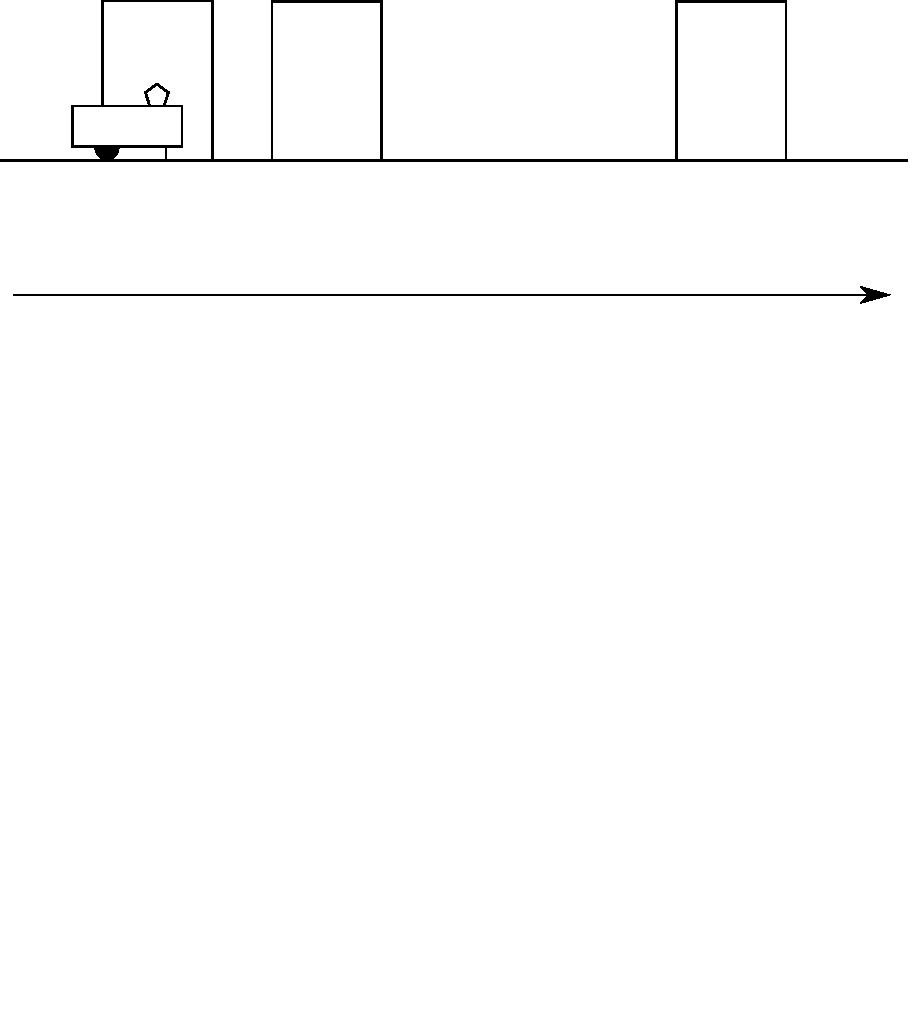
\includegraphics[width=\textwidth]{figs/three_door_example}
    \def\svgwidth{\textwidth}
    \import{./figs/}{three_door_example.pdf_tex}
	\caption{A robot localizing itself using a ``door detector'' in a known map. Top: Upon encountering a door, the robot can be in front of any of the three doors. Middle: When driving to the right, the Gaussian distributions representing its location also shift to the right and widen, representing growing uncertainty. Bottom: After detecting the second door, the robot can discard hypotheses that are not in front of the door and gains certainty on its location. }
	\label{fig:three_door_example}
\end{figure}

\section{Markov Localization}\label{sec:markovloc}
Calculating the probability to be at a certain location given the likelihood of certain observations is nothing else as a conditional probability. There is a formal way to describe such situations: Bayes' Rule (\cref{sec:bayesrule})\index{Bayes' rule}:
\begin{equation}
P(A|B)=\frac{P(A)P(B|A)}{P(B)}
\end{equation}
\subsection{Perception Update}
How does this map into a Localization framework? Let's assume, event $A$ is equivalent to be at a specific location $loc$. Lets also assume that event $B$ corresponds to the event to see a particular feature $feat$. We can now rewrite Bayes' rule to

\begin{equation}
P(loc|feat)=\frac{P(loc)P(feat|loc)}{P(feat)}
\end{equation}

Rephrasing Bayes' rule in this way, we can calculate the probability to be at location $loc$, given that we see feature $feat$. This is known as \textsl{Perception Update}\index{Perception Update (Markov Localization)}. For example, $loc$ could correspond to door 1, 2 or 3, and $feat$ could be the event of sensing a door. What do we need to know to make use of this equation?
\begin{enumerate}
\item We need to know the prior probability to be at location loc $P(loc)$
\item We need to know the probability to see the feature at this location $P(feat|loc)$
\item We need the probability to encounter the feature feat $P(feat)$
\end{enumerate}
Let's start with (3), which might be the most confusing part of information we need to collect. The answer is simple, no matter what $P(feat)$ is, it will cancel out as the probability to be at any of the possible locations has to sum up to 1. (A simpler, although less accurate, explanation would be that the probability to sense a feature is constant and therefore does not matter.)

The prior probability to be at location  $loc$, $P(loc)$, is called the \index{Belief Model} \textsl{belief model}. In the case of the 3-door example, it is the value of the Gaussian distribution underneath the door corresponding to $loc$.

Finally, we need to know the probability to see the feature $feat$ at location $loc$ $P(feat|loc)$. If your sensor were perfect, this probability is simply 1 if the feature exists at this location, or 0 if the feature cannot be observed at this location. If your sensor is not perfect, $P(feat|loc)$ corresponds to the likelihood for the sensor to see the feature if it exists.

The final missing piece is how to best represent possible locations. In the graphical example in \cref{fig:three_door_example} we assumed Gaussian distributions for each possible location. Alternatively, we can also discretize the world into a grid and calculate the likelihood of the robot to be in any of its cells. In our 3-door world, it might make sense to choose grid cells that have just the width of a door.

\subsection{Action Update}
One of the assumptions in the above thought experiment was that we know with certainty that the robot moved right. We will now more formally study how to treat uncertainty from motion. Recall that odometry input is just another sensor that we assume to have a Gaussian distribution; if our odometer tells us that the robot traveled a meter, it could have traveled a  little less or a little more, with decreasing likelihood. We can therefore calculate the posterior probability of the robot moving from a position $loc'$ to $loc$ given its odometer input $odo$:

\begin{equation}
P(loc'->loc|odo)=P(loc'->loc)P(odo|loc'->loc)/P(odo)
\end{equation}

This is again Bayes' rule. The unconditional probability $P(loc'->loc)$ is the prior probability for the robot to have been at location $loc'$. The term $ P(odo|loc'->loc)$ corresponds to the probability to get odometer reading $odo$ after traveling from a position $loc'$ to $loc$. If getting a reading of the amount $odo$ is reasonable for the distance from $loc'$ to $loc$ this probability is high. If it is unreasonable, for example if the distance is larger than what is physically possible, this probability should be very low.

As the robot's location is uncertain, the real challenge is now that the robot could have potentially been everywhere to start with. We therefore have to calculate the posterior probability $P(loc|odo)$ for all possible positions $loc'$. This can be accomplished by summing over all possible locations:
\begin{equation}
P(loc|odo)=\sum_{loc'}P(loc'->loc)P(odo|loc'->loc)
\end{equation}
In other words, the law of total probability requires us to consider all possible locations the robot could have ever been at. This step is known as \textsl{Action Update}\index{Action Update (Markov Localization)}. In practice we don't need to calculate this for all possible locations, but only those that are technically feasible given the maximum speed of the robot. We note also that the sum notation technically corresponds to a convolution (\cref{sec:convolution}) of the probability distribution of the robot's location in the environment with the robot's odometry error probability distribution.

\subsection{Summary and Examples}
We have now learned two methods to update the belief distribution of where the robot could be in the environment. First, a robot can use external landmarks to update its position. This is known as \textsl{perception update} and relies on exterioception. Second, a robot can observe its internal sensors. This is known as \textsl{action update} and relies on proprioception. The combination of action and perception updates is known as \textsl{Markov Localization}\index{Markov Localization}. You can think about the action update to increase the uncertainty of the robot's position and the perception update to shrink it. (You can also think about the action update as a discrete version of the error propagation model.) Also here we are using the robotics kinematic model and the noise model of your odometer to calculate $ P(odo|loc'->loc)$.

\paragraph{Example 1: Topological Map}
This example describes one of the first successful real robot systems that employed Markov Localization in an office environment. The experiment is described in more detail in a 1995 article of AI Magazine\cite{nourbakhsh1995dervish}. The office environment consisted of two rooms and a corridor that can be modeled by a topological map\index{Topological Map} (\cref{fig:dervish_example}). In a topological map, areas that the robot can be in are modeled as vertices, and navigable connections between them are modeled as edges of a graph. The location of the robot can now be represented as a probability distribution over the vertices of  this graph.

\begin{figure}
	\centering
	% 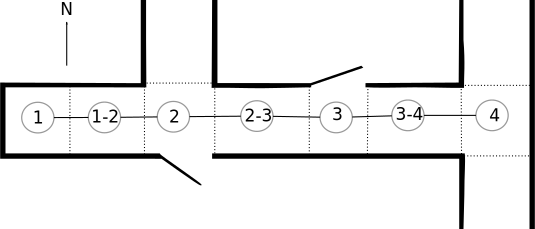
\includegraphics[width=\textwidth]{figs/dervish_example}
    \def\svgwidth{\textwidth}
    \import{./figs/}{dervish_example.pdf_tex}
	\caption{An office environment consisting of two rooms connected by a hallway. A topological map is super-imposed.}
	\label{fig:dervish_example}
\end{figure}

The robot has the following sensing abilities:
\begin{itemize}
    \item It can detect a closed door to its left or right.
    \item It can detect an open door to its left or right.
    \item It can detect whether it is an open hallway.
\end{itemize}

Unfortunately, the robot's sensors are not at all reliable. The researchers have experimentally found the probabilities to obtain a certain sensor response for specific physical positions using their robot in their environment. These values are provided in \cref{tab:dervish_example}.

\begin{table}
\footnotesize
\begin{tabular}{lccccc}
 	& Wall	& Closed dr & Open dr	& Open hwy & Foyer\\
\hline
Nothing detected	& 70\%	& 40\%&	5\%	& 0.1\% & 30\%\\
Closed door detected & 30\% &	60\%& 0\% &0\%	& 5\%\\
Open door detected & 0\%	& 0\%&	90\% & 10\% & 15\%\\
Open hallway detected & 0\% &	 0\%&	0.1\% & 90\% &50\%\\
\hline
\end{tabular}
\normalsize
\caption{Conditional probabilities of the Dervish robot detecting certain features in the Stanford laboratory.\label{tab:dervish_example}}
\end{table}

For example, the success rate to detect a closed door is only 60\%, whereas a foyer looks like an open door in 15\% of the trials. This data corresponds to the conditional probability to detect a certain feature given a certain location.

Consider now the following initial belief state distribution: $p(1-2)=0.8$ and $p(2-3)=0.2$. Here, $1-2$ etc.\ refers to the position on the topological map in \cref{fig:dervish_example}. You know that the robot faces east with certainty. The robot now drives for a while until it reports ``open hallway on its left and open door on its right''. This actually corresponds to location 2, but the robot can in fact be anywhere. For example there is a 10\% chance that the open door is in fact an open hallway, i.e.\ the robot is really at position 4. How can we calculate the new probability distribution of the robot's location? Here are the possible trajectories that could happen:

The robot could move from $2-3$ to $3$, $3-4$ and finally $4$. We have chosen this sequence as the probability to detect an open door on its right is zero for $3$ and $3-4$, which leaves position $4$ as the only option if the robot has started at $2-3$. In order for this hypothesis to be true, the following events need to have happened, their probabilities are given in parentheses:
\begin{enumerate}
    \item The robot must have started at $2-3$ (20\%)
    \item Not have seen the open door at the left of $3$ (5\%) and not have seen the wall at the right (70\%)
    \item Not have seen the wall to its left (70\%) and not have seen the wall to its right at node $3-4$ (70\%)
    \item Correctly identify the open hallway to its left (90\%) and mistake the open hallway to its right for an open door (10\%)
\end{enumerate}
Together, the likelihood that the robot got from position $2-3$ to position $4$ is therefore given by $0.2\times 0.05 \times 0.7 \times 0.7 \times 0.7 \times 0.9 \times0.1=0.03\%$, that is very unlikely.

The robot could also move from $1-2$ to $2$, $2-3$, $3$, $3-4$ or $4$. We can evaluate these hypotheses in a similar way:
\begin{itemize}
    \item The chance that it correctly detects the open hallway and door at position $2$ is $0.9 \times 0.9$, so the chance to be at position $2$, having started at $1-2$, is $0.8 \times 0.9 \times 0.9=64\%$.
    \item The robot cannot have ended up at position $2-3$, $3$, and $3-4$ because the chance of seeing an open door instead of a wall on the right side is zero in all these cases.
    \item In order to reach position $4$, the robot must have started at $1-2$ has a chance of $0.8$. The robot must not have seen the hallway on its left and the open door to its right when passing position $2$. The probability for this is $0.001 \times 0.05$. The robot must then have detected nothing at $2-3$ ($0.7 \times 0.7$), nothing at $3$ ($0.05 \times 0.7$), nothing at $3-4$ ($0.7 \times 0.7$), and finally mistaken the hallway on its right for an open door at position $4$ ($0.9 \times 0.1$). Multiplied together, this outcome is very unlikely.
\end{itemize}

Given this information, we can now calculate the posterior probability to be at a certain location on the topological map by adding up the probabilities for every possible path to get there.

\paragraph{Example 2: Grid-based Markov Localization}

\begin{figure}
	\centering
	% 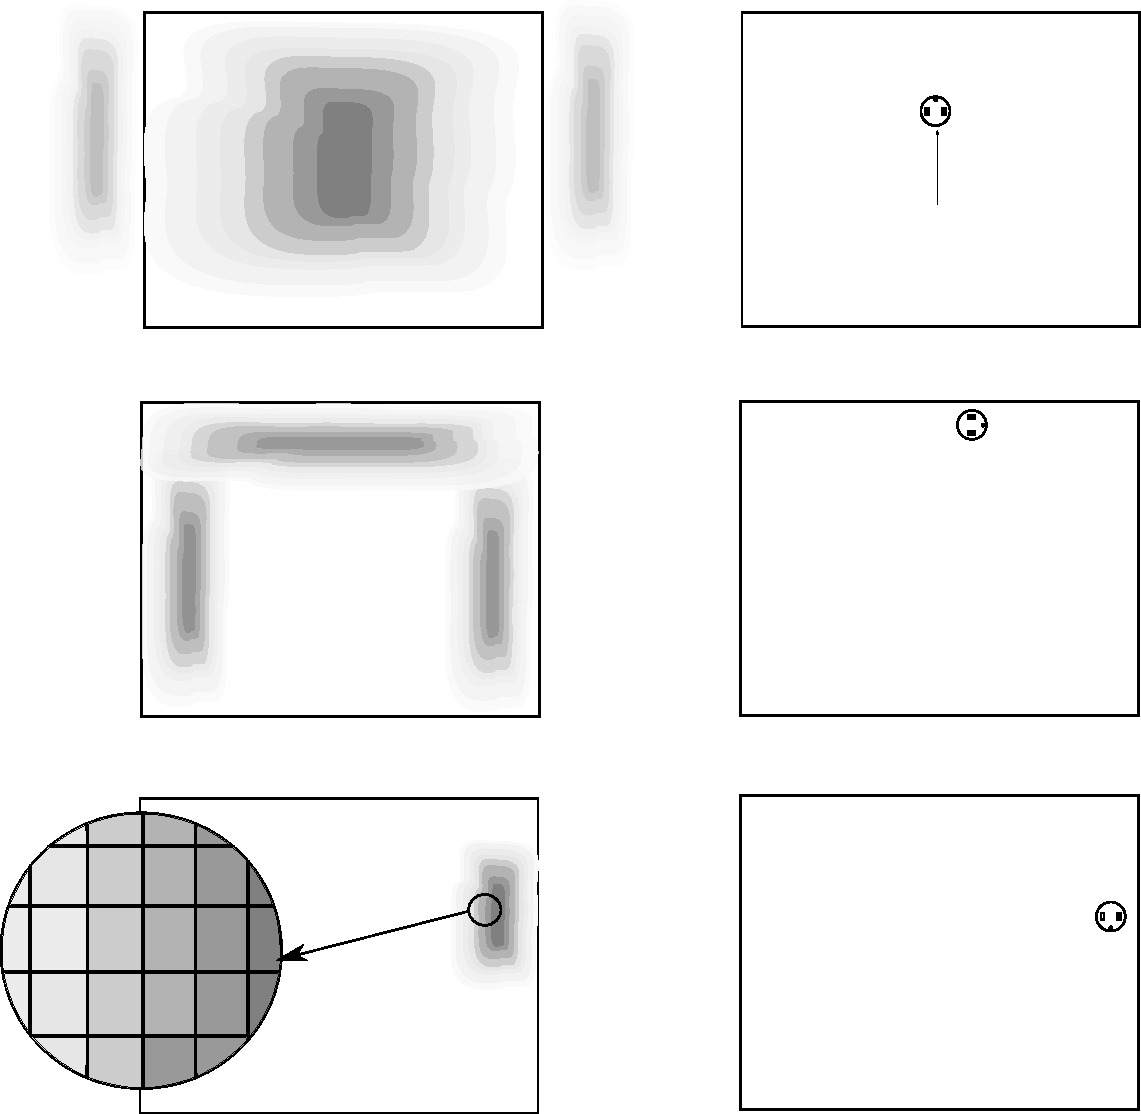
\includegraphics[width=\textwidth]{figs/markov_grid_example}
    \def\svgwidth{\textwidth}
    \import{./figs/}{markov_grid_example.pdf_tex}
	\caption{Markov localization on a grid. The left column shows the likelihood to be in a specific cell as grey value (dark colors correspond to high likelihoods). The right column shows the actual robot location. Arrows indicate previous motion. Initially, the position of the robot is unknown, but recorded upwards motion makes positions at the top of the map more likely. After the robot has encountered a wall, positions away from walls become unlikely. After rightwards and down motions, the possible positions have shrunk to a small area.}
	\label{fig:markov_grid_example}
\end{figure}

Instead of using a coarse topological map, we can also model the environment as a fine-grained grid. Each cell is marked with a probability corresponding to the likelihood of the robot being at this exact location (\cref{fig:markov_grid_example}). We assume that the robot is able to detect walls with some certainty. The images in the right column show the actual location of the robot. Initially, the robot does not see a wall and therefore could be almost anywhere. The robot now moves northwards. The action update now propagates the probability of the robot being somewhere upwards. As soon as the robot encounters the wall, the perception update bumps up the likelihood to be anywhere near a wall. As there is some uncertainty associated with the wall detector, the robot cannot only be directly at the wall, but anywhere --- with decreasing probability --- close by. As the action update involved continuous motion to the north, the likelihood to be close to the south wall is almost zero. The robot then performs a right turn and travels along the wall in clockwise direction. As soon as it hits the east wall, it is almost certain about its position, which then again decreases.

\section{Particle Filter}
Although grid-based Markov Localization can provide compelling results, it can be computationally very expensive, in particular when the environment is large and the resolution of the grid is small. This is in part due to the fact that we need to carry the probability to be at a certain location forward for every cell on the grid, regardless of how small this probability is. An elegant solution to this problem is the particle filter. It works as follows:
\begin{enumerate}
\item Represent the robot's position by $N$ particles that are randomly distributed around its estimated initial position. For this, we can either use one or more Gaussian distributions around the initial estimate(s) of where the robot is, or choose an uniform distribution (\cref{fig:particlefilter_example}).
\item Every time the robot moves, we will move each particle in the exact same way, but add noise to each movement much like we would observe on the real robot. Without a perception update, the particles will spread apart farther and farther.
\item Upon a perception event, we evaluate every single particle using our sensor model. What would the likelihood be to have a perception event such as we observed at this location? We can then use Bayes' rule to update each particle's position.
\item Once in a while or during perception events that render certain particles infeasible, particles that have a too low probability can be deleted, while those with the highest probability can be replicated.
\end{enumerate}

\begin{figure}[!htb]
	\centering
	% 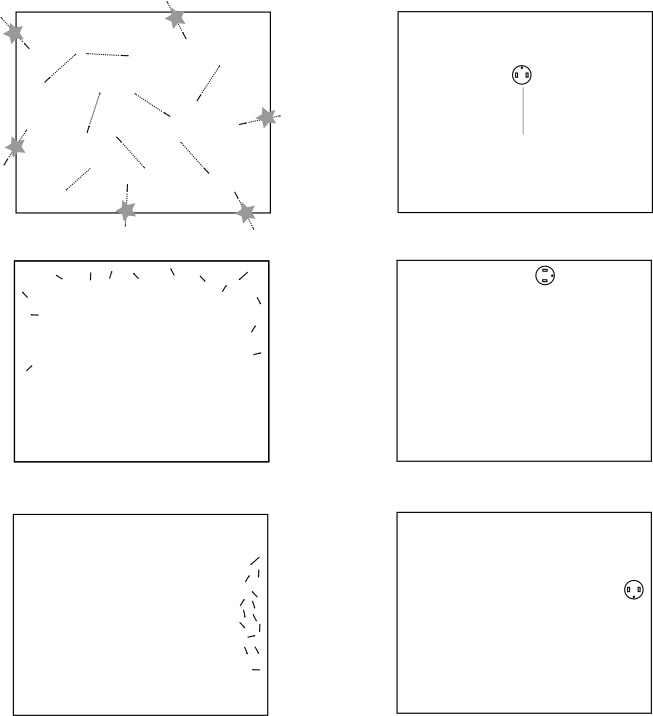
\includegraphics[width=\textwidth]{figs/particlefilter_example}
    \def\svgwidth{0.92\textwidth}
    \import{./figs/}{particlefilter_example.pdf_tex}
	\caption{Particle filter example. Possible positions and orientations of the robot are initially uniformly distributed. Particles move based on the robot's motion model. Particles that would require the robot to move through a wall in absence of a wall perception event are deleted (stars). After a perception event, particles too far of a wall become unlikely and their positions are resampled in the vicinity of a wall. Eventually, the particle filter converges.}
	\label{fig:particlefilter_example}
\end{figure}

\td{TODO: Lots of editing from the Kalman filter section.}

%\paragraph{2. Observation}
%Let us now assume that we can detect line features $ \boldsymbol{z}_{k,i}=(\alpha_i,r_i)^T$, where $ \alpha$ and $ r$ are the angle and distance of the line from the coordinate system of the robot. These line features are subject to variances $ \sigma_{\alpha,i}$ and $ \sigma_{r,i}$, which make up the diagonal of $ \boldsymbol{R}_{k}$. See the line detection section for a derivation of how angle and distance as well as their variance can be calculated from a laser scanner. The observation is a 2x1 matrix.

\paragraph{3. Measurement Update}
We assume that we can uniquely identify the lines we are seeing and retrieve their real position from a map. This is much easier for unique features, but can be done also for lines by assuming that our error is small enough and we therefore can search through our map and pick the closest lines. As features are stored in global coordinates, we need to transpose them into how the robot would see them. In practice this is nothing but a list of lines, each with an angle and a distance, but this time with respect to the origin of the global coordinate system. Transposing them into robot coordinates is straightforward. With  $ \hat{\boldsymbol{x}}_{k}=(x_{k},y_{k},\theta_k)^T$ and $ m_i=(\alpha_i,r_i)$ the corresponding entry from the map, we can write

\begin{equation} h(\hat{\boldsymbol{x}}_{k|k-1})=\left[\begin{array}{c}\alpha_{k,i}\\r_{k,i}\end{array}\right]=h(\boldsymbol{x},m_i)=\left[\begin{array}{c}\alpha_i-\theta\\r_i-(x cos(\alpha_i)+y sin(\alpha_i)\end{array}\right]
\end{equation}

and calculate its Jacobian $ \boldsymbol{H}_{k}$ as the partial derivatives of $ \alpha$ to $ x,y,\theta$ in the first row, and the partial derivatives of $ r$ in the second. How to calculate $ h()$ to predict the radius at which the robot should see the feature with radius $ r_i$ from the map is illustrated in the figure below.


%\begin{mdframed}
%Example on how to predict the distance to a feature the robot would see given its estimated position and its known location from a map.
%\end{mdframed}

\paragraph{4. Matching}
We are now equipped with a measurement $ \boldsymbol{z}_k$ and a prediction $ h(\hat{\boldsymbol{x}}_{k|k-1})$ based on all features stored in our map. We can now calculate the innovation
\begin{equation}
\tilde{\boldsymbol{y}}_{k}=\boldsymbol{z}_{k}-h(\hat{\boldsymbol{x}}_{k|k-1})
\end{equation}

which is simply the difference between each feature that we can see and those that we predict from the map. The innovation is again a 2x1 matrix.

\td{End TODO.}

\section{Probabilistic Map based localization}
In order to localize a robot using a map, we need to perform the following steps
\begin{enumerate}
\item Calculate an estimate of our new position using the forward kinematics and knowledge of the wheel-speeds that we sent to the robot until the robot encounters some uniquely identifiable feature.
\item Calculate the relative position of the feature (a wall, a landmark or beacon) to the robot.
\item Use knowledge of where the feature is located in global coordinates to predict what the robot should see.
\item Calculate the difference between what the robot actually sees and what it believes it should see (e.g.\ using a Kalman filter).
\item Use the result from (4) to update its belief by weighing each observation with its variance.
\end{enumerate}

Steps 1-2 are based on the sections on ``Forward Kinematics'' and ``Line detection''. Step 3 uses again simple forward kinematics to calculate the position of a feature stored in global coordinates in a map in robot coordinates. Step 4 is a simple subtraction of what the sensor sees and what the map says. Step 5 may induce the Kalman filter, or an error minimization constraint, which we will describe here. Its derivation is involved, but its intuition is simple: why just averaging between where I think I am and what my sensors tell me, if my sensors are much more reliable and should carry much higher weight?


\section*{Take home lessons}
\begin{itemize}
\item If the robot has no additional sensors and its odometry is noisy, error propagation will lead to ever increasing uncertainty of a robot's position regardless of using Markov localization or the Kalman filter.
\item Once the robot is able to sense features with known locations, Bayes' rule can be used to update the posterior probability of a possible position. The key insight is that the conditional probability to be at a certain position given a certain observation can be inferred from the likelihood to actually make this observation given a certain position.
\item A complete solution that performs this process for discrete locations is known as Markov Localization.
\item The Extended Kalman Filter is the optimal way to fuse observations of different random variables that are Gaussian distributed.
It is derived by minimizing the least-square error between prediction and real value.
\item Possible random variables could be the estimate of your robot position from odometry and observations of static beacons with known location (but uncertain sensing) in the environment.
\item In order to take advantage of the approach, you will need differentiable functions that relate measurements to state variables as well as an estimate of the covariance matrix of your sensors.
\item An approximation that combines benefits of Markov Localization (multiple hypothesis) and the Kalman filter (continuous representation of position estimates) is the Particle filter.
\end{itemize}

\section*{Exercises}\small
\begin{enumerate}
\item Assume that the ceiling is equipped with infra-red markers that the robot can identify with some certainty. Your task is to develop a probabilistic localization scheme, and you would like to calculate the probability $p(marker|reading)$ to be close to a certain marker given a certain sensing reading and information about how the robot has moved.
\begin{enumerate}
\item Derive an expression for $p(marker|reading)$ assuming that you have an estimate of the probability to correctly identify a marker $p(reading|marker)$ and the probability $p(marker)$ of being underneath a specific marker.
\item Now assume that the likelihood that you are reading a marker correctly is 90\%, that you get a wrong reading is 10\%, and that you do not see a marker when passing right underneath it is 50\%. Consider a narrow corridor that is equipped with 4 markers. You know with certainty that you started from the entry closest to marker 1 and move right in a straight line. The first reading you get is ``Marker 3''. Calculate the probability to be indeed underneath marker 3.
\item Could the robot also possibly be underneath marker 4?
\end{enumerate}

\end{enumerate}\normalsize
